%%%%%%%%%%%%%%%%%%%%%%%%%%%%%%%%%%%%%%%%%
% Beamer Presentation
% LaTeX Template
% Version 1.0 (10/11/12)
%
% This template has been downloaded from:
% http://www.LaTeXTemplates.com
%
% License:
% CC BY-NC-SA 3.0 (http://creativecommons.org/licenses/by-nc-sa/3.0/)
%
%%%%%%%%%%%%%%%%%%%%%%%%%%%%%%%%%%%%%%%%%

%----------------------------------------------------------------------------------------
%	PACKAGES AND THEMES
%----------------------------------------------------------------------------------------

\documentclass{beamer}

\mode<presentation> {

% The Beamer class comes with a number of default slide themes
% which change the colors and layouts of slides. Below this is a list
% of all the themes, uncomment each in turn to see what they look like.

%\usetheme{default}
%\usetheme{AnnArbor}
%\usetheme{Antibes}
%\usetheme{Bergen}
%\usetheme{Berkeley}
%\usetheme{Berlin}
%\usetheme{Boadilla}
\usetheme{CambridgeUS}
%\usetheme{Copenhagen}
%\usetheme{Darmstadt}
%\usetheme{Dresden}
%\usetheme{Frankfurt}
%\usetheme{Goettingen}
%\usetheme{Hannover}
%\usetheme{Ilmenau}
%\usetheme{JuanLesPins}
%\usetheme{Luebeck}
%\usetheme{Madrid}
%\usetheme{Malmoe}
%\usetheme{Marburg}
%\usetheme{Montpellier}
%\usetheme{PaloAlto}
%\usetheme{Pittsburgh}
%\usetheme{Rochester}
%\usetheme{Singapore}
%\usetheme{Szeged}
%\usetheme{Warsaw}

% As well as themes, the Beamer class has a number of color themes
% for any slide theme. Uncomment each of these in turn to see how it
% changes the colors of your current slide theme.

%\usecolortheme{albatross}
%\usecolortheme{beaver}
%\usecolortheme{beetle}
%\usecolortheme{crane}
%\usecolortheme{dolphin}
%\usecolortheme{dove}
%\usecolortheme{fly}
%\usecolortheme{lily}
%\usecolortheme{orchid}
%\usecolortheme{rose}
%\usecolortheme{seagull}
\usecolortheme{seahorse}
%\usecolortheme{whale}
%\usecolortheme{wolverine}

%\setbeamertemplate{footline} % To remove the footer line in all slides uncomment this line
\setbeamertemplate{footline}[page number] % To replace the footer line in all slides with a simple slide count uncomment this line

\setbeamertemplate{navigation symbols}{} % To remove the navigation symbols from the bottom of all slides uncomment this line

%\setbeamercolor{block title}{bg=olive}
}

\usepackage{graphicx} % Allows including images
\usepackage{booktabs} % Allows the use of \toprule, \midrule and \bottomrule in tables


%\usepackage{sty/lstlang0}
%\usepackage{texments}
\usepackage{listings}
\usepackage{color}

% "define" Scala
\lstdefinelanguage{scala}{
  morekeywords={abstract,case,catch,class,def,%
    do,else,extends,false,final,finally,%
    for,if,implicit,import,match,mixin,%
    new,null,object,override,package,%
    private,protected,requires,return,sealed,%
    super,this,throw,trait,true,try,%
    type,val,var,while,with,yield},
  otherkeywords={=>,<-,<\%,<:,>:,\#,@},
  sensitive=true,
  morecomment=[l]{//},
  morecomment=[n]{/*}{*/},
  morestring=[b]",
  morestring=[b]',
  morestring=[b]"""
}

\usepackage{color}
\definecolor{dkgreen}{rgb}{0,0.6,0}
\definecolor{gray}{rgb}{0.5,0.5,0.5}
\definecolor{mauve}{rgb}{0.58,0,0.82}

\lstset{frame=tb,
  language=scala,
  aboveskip=3mm,
  belowskip=3mm,
  showstringspaces=false,
  columns=flexible,
  basicstyle={\small\ttfamily},
  numbers=none,
  numberstyle=\tiny\color{gray},
  keywordstyle=\color{blue},
  commentstyle=\color{dkgreen},
  stringstyle=\color{mauve},
  frame=single,
  breaklines=true,
  breakatwhitespace=true
  tabsize=3
}


 
\newcommand{\TCR}{\textcolor{red}}
\newcommand{\TCG}{\textcolor{green}}
\newcommand{\TCB}{\textcolor{blue}}
\newcommand{\TCM}{\textcolor{brown}}
\definecolor{applegreen}{rgb}{0.10, 0.40, 0.20}
\newcommand{\TCAG}{\textcolor{applegreen}}


%----------------------------------------------------------------------------------------
%	TITLE PAGE
%----------------------------------------------------------------------------------------

\title[Direct Embedding]{Direct Embedding} % The short title appears at the bottom of every slide, the full title is only on the title page

\author{Joris Beau} % Your name
\institute[EPFL] % Your institution as it will appear on the bottom of every slide, may be shorthand to save space
{
EPFL - LAMP \\ % Your institution for the title page
Project in computer science\\


Directed by \textbf{Martin Odersky}, Supervised by \textbf{Vojin Jovanovic}\\
\subject{Computer Science}
\medskip
%\textit{john@smith.com} % Your email address
}
\date{\today} % Date, can be changed to a custom date

\begin{document}
%\lstset{language=Java} 

\begin{frame}
\titlepage % Print the title page as the first slide
\end{frame}

%------------------------------------------------
\section{Introduction} % Sections can be created in order to organize your presentation into discrete blocks, all sections and subsections are automatically printed in the table of contents as an overview of the talk
%------------------------------------------------

\subsection{Motivation, Goal \& Features } % A subsection can be created just before a set of slides with a common theme to further break down your presentation into chunks

\begin{frame}[fragile]
\frametitle{Motivation}

\centerline{As a DSL author...}

\end{frame}

%------------------------------------------------

\begin{frame}[fragile]
\frametitle{Motivation}

\centerline{would you like to write this kind of code?}
\begin{lstlisting}
t.symbol.owner.isType
&& t.symbol.owner.asType == typeOf[ch.epfl.__.__.type].typeSymbol
&& x.symbol.name.toString == "query"
...
\end{lstlisting}

\centerline{OR}
\begin{lstlisting}
case Query ...
\end{lstlisting}


\end{frame}

%------------------------------------------------

\begin{frame}
\frametitle{Outline} % Table of contents slide, comment this block out to remove it
\tableofcontents
\end{frame}

%------------------------------------------------

\begin{frame}[fragile]
\frametitle{Motivation}
\begin{itemize}
\item Instigated by Slick database library
\item Embedding DSLs simply!
\item Provide a painless logic for reification
\item Direct embedding has avantages:\\
	- better error messages\\
	- compile-time\\
\end{itemize}

%\pygment{sh}{



\end{frame}

%------------------------------------------------

\begin{frame}
\frametitle{Goal}
\begin{itemize}
\item Educational aspect
\item Implement a core prototype
\item Make it work \& extend it
\item Apply on real examples
\item Might evolve to a complete library
\end{itemize}
\end{frame}


%------------------------------------------------

\begin{frame}
\frametitle{Features}

\centerline{Users' friendly}
\begin{itemize}
\item Scala-like language in Scala projects
\item Take care of difficulties (macro)
\item Provide easy and general tool
\item Avoid complex and too specific code
\end{itemize}

\end{frame}

%------------------------------------------------
%------------------------------------------------
\subsection{Context}

\begin{frame}
\frametitle{Big Picture of Slick}

\begin{figure}
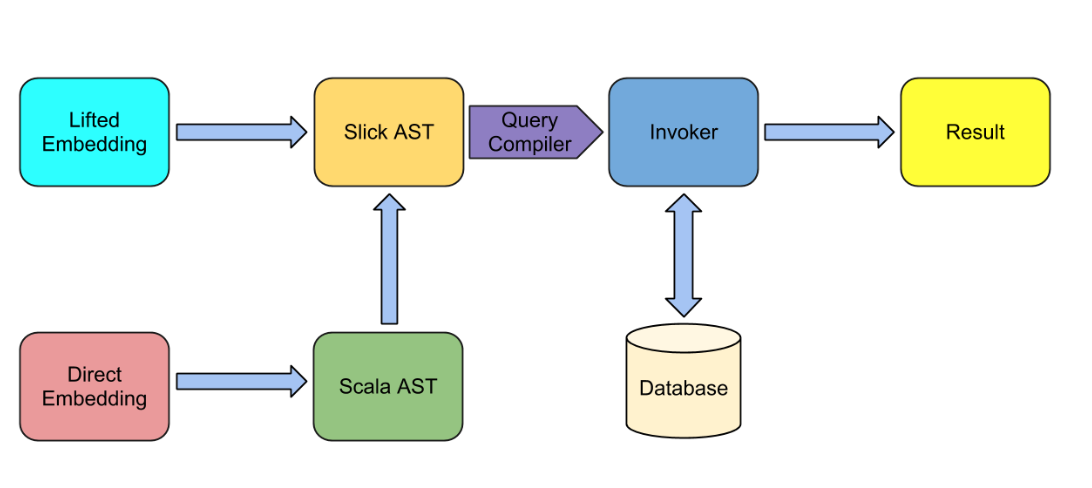
\includegraphics[width=0.8\linewidth]{./img/bigp.png}
\end{figure}

\end{frame}

%------------------------------------------------


\begin{frame}
\frametitle{Direct embedding aspects}

\begin{itemize}
\item AST generated compile-time 
\item macro based
\item Scala type
\item at runtime, errors for unsupported methods
\item  experimental on Slick
\end{itemize}

\end{frame}

%------------------------------------------------
\section{Implementation}
%------------------------------------------------
%------------------------------------------------
\subsection{Reification}

\begin{frame}[fragile]
\frametitle{Reification: Need to modify Scala AST}

$\mathbf{Recall}$: we want to avoid this kind of ugly and specific code
\begin{lstlisting}
t.symbol.owner.isType
&& t.symbol.owner.asType == typeOf[ch.epfl.__.__.type].typeSymbol
&& x.symbol.name.toString == "query"
\end{lstlisting}


\end{frame}

%------------------------------------------------


\begin{frame}[fragile]
\frametitle{Reification: Need to modify Scala AST}

What do we want, exactly?
\begin{itemize}
\item Write simple code, 
\item without knowledge about the DSL aspects,
\item but that is for DSL
\end{itemize}

Let us write it and let someone else take care of details


\end{frame}

%------------------------------------------------


\begin{frame}[fragile]
\frametitle{Reification: Need to modify Scala AST}

Let us thinking on an example:
\begin{lstlisting}
 def query[T](q:QueryableValue[T]) = ...
 val coffees = Queryable[Coffee]
 \end{lstlisting}
 
But here \TCR{Coffee} refers to a SQL table...\\
We need to specify it without knowledge about the domain and without huge overhead\\
Intermediate Representation (IR):\\

\begin{lstlisting}
 case class Coffee(...) // where Coffee will refer to SQL table
\end{lstlisting}
 Later on we will examine the IR and transform the corresponding AST

\end{frame}

%------------------------------------------------

\begin{frame}
\frametitle{Beginning with AST}

How to modify Scala AST?\\

\end{frame}

%------------------------------------------------

\begin{frame}
\frametitle{Quasiquote}

How to modify Scala AST?\\
$\rightarrow $ \textbf{quasiquote?}\\

\end{frame}


%------------------------------------------------

\begin{frame}
\frametitle{No quasiquote}
\begin{columns}[c] % The "c" option specifies centered vertical alignment while the "t" option is used for top vertical alignment

\column{.45\textwidth} % Left column and width
\textbf{No quasiquote}
because of AST output is not fixe
\column{.5\textwidth} % Right column and width
but ...
\end{columns}
\end{frame}

%------------------------------------------------

\begin{frame}
\frametitle{Symbols}
\begin{columns}[c] % The "c" option specifies centered vertical alignment while the "t" option is used for top vertical alignment

\column{.30\textwidth} % Left column and width
\textbf{but}\\
we can access to the symbols 

\column{.05\textwidth} % Left column and width
$\rightarrow$

\column{.45\textwidth} % Right column and width
~ \TCR{@ANNOTATIONS}

\end{columns}
\end{frame}

%------------------------------------------------

\begin{frame}[fragile]
\frametitle{Annotation}

\begin{lstlisting}
@table("COFFEES") // the annotation
case class Coffee(    // the IR
...
)
\end{lstlisting}

\end{frame}

\subsection{Simple cases prototype}

%------------------------------------------------

\begin{frame}
\frametitle{Overview}
\begin{figure}
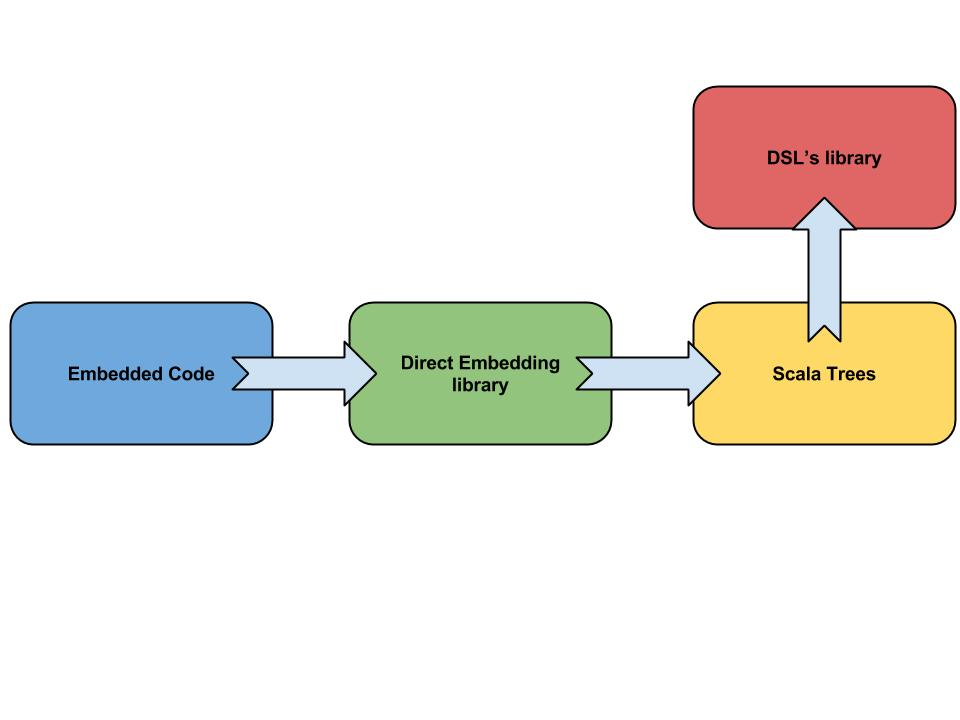
\includegraphics[width=0.8\linewidth]{./img/flow.jpg}
\end{figure}
\end{frame}

%------------------------------------------------

\begin{frame}[fragile]
\frametitle{Macro}

\begin{lstlisting}
@table("COFFEES")
case class Coffee(
    @column("COF_NAME")
    name: String,
    @column("PRICE")
    price: Double
)
\end{lstlisting}

\begin{block}{Tree}
 Apply(Select(New(Ident(ch.epfl.directembedding.test.ClassExample)), termNames.CONSTRUCTOR), List())
\end{block}

\end{frame}

%------------------------------------------------

\begin{frame}[fragile]
\frametitle{Result idea}

From symbol, arguments, type, we can use the annotation to reify the tree:
\begin{block}{Macro}
 $\implies$ macro q"..." 
\end{block}

\begin{block}{Return}
 \TCB{table}(name: \TCB{column}[\TCR{String}], price: \TCB{column}[\TCR{Double}])
\end{block}

\end{frame}

%------------------------------------------------

\begin{frame}
\frametitle{Summary of the example}

\begin{itemize}
\item Users accordingly annotate DSLs expressions
\item ASTs generated and transformed via macro
\item After the modification, the tree contains the DSL representation .i.e. the annotation
\end{itemize}

\end{frame}

%------------------------------------------------

\begin{frame}
\frametitle{Objects}
\begin{table}
\begin{tabular}{lccc}
\toprule
Cases & Object & Nested & Classes\\
\midrule
\TCR{val} \TCAG{value} & \TCG{$\checkmark$} & \TCG{$\checkmark$} & \TCG{$\checkmark$} \\
\TCR{def} \TCAG{foo} & \TCG{$\checkmark$} & \TCG{$\checkmark$} & \TCG{$\checkmark$} \\
\TCR{def} \TCAG{foo}(args) & \TCG{$\checkmark$} & \TCG{$\checkmark$} & \TCG{$\checkmark$} \\
\TCR{def} \TCAG{foo}[T, U]: (T, U) & \TCG{$\checkmark$} & \TCG{$\checkmark$} & \TCG{$\checkmark$} \\
\TCR{def} \TCAG{foo}[T, U](t: T, u: U): (T, U) & \TCG{$\checkmark$} & \TCG{$\checkmark$} & \TCG{$\checkmark$} \\
\TCR{def} \TCAG{foo}[T](t$_1$: T)(...)(t$_a$: T) & \TCG{$\checkmark$} & \TCG{$\checkmark$} & \TCG{$\checkmark$} \\
\bottomrule
\end{tabular}
%\caption{Table caption}
\end{table}
\end{frame}

%------------------------------------------------

\begin{frame}
\frametitle{Language specification}

\begin{table}
\begin{tabular}{lc}
\toprule
%Cases & \\
\midrule
%if & \TCG{$\checkmark$} \\
if & \TCR{$X$} \\
while & \TCR{$X$} \\
do while & \TCR{$X$} \\
lazy val & \TCR{$X$} \\
return & \TCR{$X$} \\
\bottomrule
\end{tabular}
%\caption{Table caption}
\end{table}
\end{frame}

%------------------------------------------------

%------------------------------------------------

\begin{frame}
\frametitle{Going further}

\begin{itemize}
\item Operator
\item Recursion
\item Raw block of code
\end{itemize}

\end{frame}

%------------------------------------------------
\section{Demonstration}
\begin{frame}
\Huge{\centerline{Demonstration}}
\end{frame}

%------------------------------------------------

\begin{frame}
\Huge{\centerline{Thank you}}
\end{frame}

%------------------------------------------------

\begin{frame}
\Huge{\centerline{Special thanks}}
\end{frame}

%------------------------------------------------

%\begin{frame}[fragile] % Need to use the fragile option when verbatim is used in the slide
%\frametitle{Citation}
%An example of the \verb|\cite| command to cite within the presentation:\\~
%
%This statement requires citation \cite{p1}.
%\end{frame}

%------------------------------------------------

%\begin{frame}
%\frametitle{References}
%\footnotesize{
%\begin{thebibliography}{99} % Beamer does not support BibTeX so references must be inserted manually as below
%\bibitem[Smith, 2012]{p1} John Smith (2012)
%\newblock Title of the publication
%\newblock \emph{Journal Name} 12(3), 45 -- 678.
%\end{thebibliography}
%}
%\end{frame}

%------------------------------------------------

%\begin{frame}[fragile] % Need to use the fragile option when verbatim is used in the slide
%\frametitle{Verbatim}
%\begin{block}{...}[Theorem Slide Code]
%\begin{verbatim}
%\begin{frame}
%\frametitle{Theorem}
%\begin{theorem}[Mass--energy equivalence]
%$E = mc^2$
%\end{theorem}
%\end{frame}\end{verbatim}
%\end{block}{...}
%\end{frame}

%----------------------------------------------------------------------------------------

\end{document} 